\documentclass[a4paper]{book}
\usepackage{a4wide}
\usepackage{makeidx}
\usepackage{fancyhdr}
\usepackage{graphicx}
\usepackage{multicol}
\usepackage{float}
\usepackage{textcomp}
\usepackage{alltt}
\usepackage{times}
\usepackage{ifpdf}
\ifpdf
\usepackage[pdftex,
            pagebackref=true,
            colorlinks=true,
            linkcolor=blue,
            unicode
           ]{hyperref}
\else
\usepackage[ps2pdf,
            pagebackref=true,
            colorlinks=true,
            linkcolor=blue,
            unicode
           ]{hyperref}
\usepackage{pspicture}
\fi
\usepackage[utf8]{inputenc}
\usepackage{doxygen}
\makeindex
\setcounter{tocdepth}{1}
\renewcommand{\footrulewidth}{0.4pt}
\begin{document}
\begin{titlepage}
\vspace*{7cm}
\begin{center}
{\Large TopUtils\_\-Tools \\[1ex]\large 1.0 }\\
\vspace*{1cm}
{\large Generated by Doxygen 1.5.5}\\
\vspace*{0.5cm}
{\small Wed Apr 15 08:57:20 2009}\\
\end{center}
\end{titlepage}
\clearemptydoublepage
\pagenumbering{roman}
\tableofcontents
\clearemptydoublepage
\pagenumbering{arabic}
\chapter{Deprecated List}
\label{deprecated__deprecated000001}
\hypertarget{deprecated__deprecated000001}{}
 \begin{description}
\item[Member \hyperlink{classtools_1_1XMLConfigParser_1_1OptionSet_6c3e2b6ef7030f2f9525bb52de68531d}{tools::XMLConfigParser::OptionSet::setDefaults} ]: will be deleted \end{description}

\chapter{Class Index}
\section{Class Hierarchy}
This inheritance list is sorted roughly, but not completely, alphabetically:\begin{CompactList}
\item \contentsline{section}{tools::XMLConfigParser::ConfigError}{\pageref{classtools_1_1XMLConfigParser_1_1ConfigError}}{}
\item \contentsline{section}{tools::XMLConfigParser::ConfigObject}{\pageref{classtools_1_1XMLConfigParser_1_1ConfigObject}}{}
\begin{CompactList}
\item \contentsline{section}{tools::XMLConfigParser::Input}{\pageref{classtools_1_1XMLConfigParser_1_1Input}}{}
\end{CompactList}
\item \contentsline{section}{tools::XMLConfigParser::Configuration}{\pageref{classtools_1_1XMLConfigParser_1_1Configuration}}{}
\item \contentsline{section}{tools::ConfigWrapper::ConfigWrapper}{\pageref{classtools_1_1ConfigWrapper_1_1ConfigWrapper}}{}
\item \contentsline{section}{tools::doxypy::FSM}{\pageref{classtools_1_1doxypy_1_1FSM}}{}
\item \contentsline{section}{tools::DrawHelper::Helper}{\pageref{classtools_1_1DrawHelper_1_1Helper}}{}
\item \contentsline{section}{tools::XMLConfigParser::OptionSet}{\pageref{classtools_1_1XMLConfigParser_1_1OptionSet}}{}
\item \contentsline{section}{tools::PadService::PadService}{\pageref{classtools_1_1PadService_1_1PadService}}{}
\item \contentsline{section}{tools::testConfigParser::testConfigParser}{\pageref{classtools_1_1testConfigParser_1_1testConfigParser}}{}
\item \contentsline{section}{tools::testXMLParser::TestParser}{\pageref{classtools_1_1testXMLParser_1_1TestParser}}{}
\end{CompactList}

\chapter{Class Index}
\section{Class List}
Here are the classes, structs, unions and interfaces with brief descriptions:\begin{CompactList}
\item\contentsline{section}{\hyperlink{classtools_1_1XMLConfigParser_1_1ConfigError}{tools::XMLConfigParser::ConfigError} (A simple Exception implementations for customized errors )}{\pageref{classtools_1_1XMLConfigParser_1_1ConfigError}}{}
\item\contentsline{section}{\hyperlink{classtools_1_1XMLConfigParser_1_1ConfigObject}{tools::XMLConfigParser::ConfigObject} (An simple configurable object )}{\pageref{classtools_1_1XMLConfigParser_1_1ConfigObject}}{}
\item\contentsline{section}{\hyperlink{classtools_1_1XMLConfigParser_1_1Configuration}{tools::XMLConfigParser::Configuration} (The definitions of the configuration )}{\pageref{classtools_1_1XMLConfigParser_1_1Configuration}}{}
\item\contentsline{section}{\hyperlink{classtools_1_1ConfigWrapper_1_1ConfigWrapper}{tools::ConfigWrapper::ConfigWrapper} (----------------------------------------------------------------------------------- wrapper class for a cfg to python transition twiki: \href{https://twiki.cern.ch/twiki/bin/view/CMS/ConfigRunner#ConfigWrapper}{\tt https://twiki.cern.ch/twiki/bin/view/CMS/ConfigRunner\#ConfigWrapper} )}{\pageref{classtools_1_1ConfigWrapper_1_1ConfigWrapper}}{}
\item\contentsline{section}{\hyperlink{classtools_1_1doxypy_1_1FSM}{tools::doxypy::FSM} (Implements a finite state machine )}{\pageref{classtools_1_1doxypy_1_1FSM}}{}
\item\contentsline{section}{\hyperlink{classtools_1_1DrawHelper_1_1Helper}{tools::DrawHelper::Helper} (Tool for the layout of histograms )}{\pageref{classtools_1_1DrawHelper_1_1Helper}}{}
\item\contentsline{section}{\hyperlink{classtools_1_1XMLConfigParser_1_1Input}{tools::XMLConfigParser::Input} (Defines an input for a histogram : does not know anything about files )}{\pageref{classtools_1_1XMLConfigParser_1_1Input}}{}
\item\contentsline{section}{\hyperlink{classtools_1_1XMLConfigParser_1_1OptionSet}{tools::XMLConfigParser::OptionSet} (Stores the options of an \hyperlink{classtools_1_1XMLConfigParser_1_1ConfigObject}{ConfigObject} and their defaults )}{\pageref{classtools_1_1XMLConfigParser_1_1OptionSet}}{}
\item\contentsline{section}{\hyperlink{classtools_1_1PadService_1_1PadService}{tools::PadService::PadService} (Builds canvas up to 6 hists )}{\pageref{classtools_1_1PadService_1_1PadService}}{}
\item\contentsline{section}{\hyperlink{classtools_1_1testConfigParser_1_1testConfigParser}{tools::testConfigParser::testConfigParser} (A test class for the ConfigParser module )}{\pageref{classtools_1_1testConfigParser_1_1testConfigParser}}{}
\item\contentsline{section}{\hyperlink{classtools_1_1testXMLParser_1_1TestParser}{tools::testXMLParser::TestParser} (TestCase for the XMLConfigParser )}{\pageref{classtools_1_1testXMLParser_1_1TestParser}}{}
\end{CompactList}

\chapter{Class Documentation}
\hypertarget{classtools_1_1XMLConfigParser_1_1ConfigError}{
\section{tools::XMLConfigParser::ConfigError Class Reference}
\label{classtools_1_1XMLConfigParser_1_1ConfigError}\index{tools::XMLConfigParser::ConfigError@{tools::XMLConfigParser::ConfigError}}
}
A simple Exception implementations for customized errors.  


\subsection*{Public Member Functions}
\begin{CompactItemize}
\item 
def \hyperlink{classtools_1_1XMLConfigParser_1_1ConfigError_70c57c0779ed34d7057a24cf494bb1a5}{\_\-\_\-init\_\-\_\-}
\begin{CompactList}\small\item\em constructor \item\end{CompactList}\item 
\hypertarget{classtools_1_1XMLConfigParser_1_1ConfigError_323776592168d84916d52a6ae9d2ca34}{
def \textbf{\_\-\_\-str\_\-\_\-}}
\label{classtools_1_1XMLConfigParser_1_1ConfigError_323776592168d84916d52a6ae9d2ca34}

\end{CompactItemize}
\subsection*{Public Attributes}
\begin{CompactItemize}
\item 
\hypertarget{classtools_1_1XMLConfigParser_1_1ConfigError_216fc30daa4058b1f6605e95a25f5b74}{
\textbf{value}}
\label{classtools_1_1XMLConfigParser_1_1ConfigError_216fc30daa4058b1f6605e95a25f5b74}

\end{CompactItemize}


\subsection{Detailed Description}
A simple Exception implementations for customized errors. 

\subsection{Member Function Documentation}
\hypertarget{classtools_1_1XMLConfigParser_1_1ConfigError_70c57c0779ed34d7057a24cf494bb1a5}{
\index{tools::XMLConfigParser::ConfigError@{tools::XMLConfigParser::ConfigError}!\_\-\_\-init\_\-\_\-@{\_\-\_\-init\_\-\_\-}}
\index{\_\-\_\-init\_\-\_\-@{\_\-\_\-init\_\-\_\-}!tools::XMLConfigParser::ConfigError@{tools::XMLConfigParser::ConfigError}}
\subsubsection{\setlength{\rightskip}{0pt plus 5cm}def tools::XMLConfigParser::ConfigError::\_\-\_\-init\_\-\_\- ( {\em self}, \/   {\em value})}}
\label{classtools_1_1XMLConfigParser_1_1ConfigError_70c57c0779ed34d7057a24cf494bb1a5}


constructor 

\begin{Desc}
\item[Parameters:]
\begin{description}
\item[{\em value,:}]an error value \end{description}
\end{Desc}


The documentation for this class was generated from the following file:\begin{CompactItemize}
\item 
XMLConfigParser.py\end{CompactItemize}

\hypertarget{classtools_1_1XMLConfigParser_1_1ConfigObject}{
\section{tools::XMLConfigParser::ConfigObject Class Reference}
\label{classtools_1_1XMLConfigParser_1_1ConfigObject}\index{tools::XMLConfigParser::ConfigObject@{tools::XMLConfigParser::ConfigObject}}
}
An simple configurable object.  


Inheritance diagram for tools::XMLConfigParser::ConfigObject::\begin{figure}[H]
\begin{center}
\leavevmode
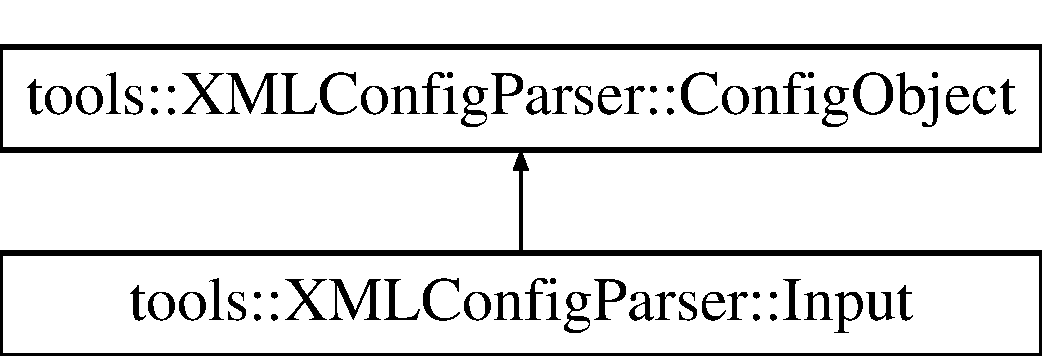
\includegraphics[height=2cm]{classtools_1_1XMLConfigParser_1_1ConfigObject}
\end{center}
\end{figure}
\subsection*{Public Member Functions}
\begin{CompactItemize}
\item 
def \hyperlink{classtools_1_1XMLConfigParser_1_1ConfigObject_da2c248a8db2c816f489af71f314c37c}{\_\-\_\-init\_\-\_\-}
\begin{CompactList}\small\item\em The standard constructor. \item\end{CompactList}\item 
\hypertarget{classtools_1_1XMLConfigParser_1_1ConfigObject_0862df3a12f28c29566910ad410ab308}{
def \textbf{setOption}}
\label{classtools_1_1XMLConfigParser_1_1ConfigObject_0862df3a12f28c29566910ad410ab308}

\item 
def \hyperlink{classtools_1_1XMLConfigParser_1_1ConfigObject_74b01910a3f928e337b2ee658ddea97b}{getOption}
\item 
\hypertarget{classtools_1_1XMLConfigParser_1_1ConfigObject_09d996cb6905edb9b830fac3564c02aa}{
def \textbf{readDefaults}}
\label{classtools_1_1XMLConfigParser_1_1ConfigObject_09d996cb6905edb9b830fac3564c02aa}

\item 
\hypertarget{classtools_1_1XMLConfigParser_1_1ConfigObject_f6cf63837cff0257365350121dfe17bb}{
def \hyperlink{classtools_1_1XMLConfigParser_1_1ConfigObject_f6cf63837cff0257365350121dfe17bb}{parseFromNode}}
\label{classtools_1_1XMLConfigParser_1_1ConfigObject_f6cf63837cff0257365350121dfe17bb}

\begin{CompactList}\small\item\em gets all attributes of the node and textnodes which are not in \char`\"{}doNotParse\char`\"{} and and adds them as options \item\end{CompactList}\end{CompactItemize}
\subsection*{Public Attributes}
\begin{CompactItemize}
\item 
\hypertarget{classtools_1_1XMLConfigParser_1_1ConfigObject_00284e82b6ab5406ca91d6ffb33e4ddf}{
\textbf{rootName}}
\label{classtools_1_1XMLConfigParser_1_1ConfigObject_00284e82b6ab5406ca91d6ffb33e4ddf}

\item 
\hypertarget{classtools_1_1XMLConfigParser_1_1ConfigObject_dbe854fff96e72df0ab11f74463e0df4}{
\textbf{doNotParse}}
\label{classtools_1_1XMLConfigParser_1_1ConfigObject_dbe854fff96e72df0ab11f74463e0df4}

\item 
\hypertarget{classtools_1_1XMLConfigParser_1_1ConfigObject_8c642c6b47664723d47fbb5d3beb406f}{
\textbf{options}}
\label{classtools_1_1XMLConfigParser_1_1ConfigObject_8c642c6b47664723d47fbb5d3beb406f}

\item 
\hypertarget{classtools_1_1XMLConfigParser_1_1ConfigObject_69bde8a5db8dfe812abb2e0f411c5c9d}{
\textbf{mandatoryObjects}}
\label{classtools_1_1XMLConfigParser_1_1ConfigObject_69bde8a5db8dfe812abb2e0f411c5c9d}

\item 
\hypertarget{classtools_1_1XMLConfigParser_1_1ConfigObject_bcca5d83893ea94d5644bb1af1b67f53}{
\textbf{subobjects}}
\label{classtools_1_1XMLConfigParser_1_1ConfigObject_bcca5d83893ea94d5644bb1af1b67f53}

\end{CompactItemize}


\subsection{Detailed Description}
An simple configurable object. 

\subsection{Member Function Documentation}
\hypertarget{classtools_1_1XMLConfigParser_1_1ConfigObject_da2c248a8db2c816f489af71f314c37c}{
\index{tools::XMLConfigParser::ConfigObject@{tools::XMLConfigParser::ConfigObject}!\_\-\_\-init\_\-\_\-@{\_\-\_\-init\_\-\_\-}}
\index{\_\-\_\-init\_\-\_\-@{\_\-\_\-init\_\-\_\-}!tools::XMLConfigParser::ConfigObject@{tools::XMLConfigParser::ConfigObject}}
\subsubsection{\setlength{\rightskip}{0pt plus 5cm}def tools::XMLConfigParser::ConfigObject::\_\-\_\-init\_\-\_\- ( {\em self}, \/   {\em rootNodeName} = {\tt \char`\"{}\char`\"{}}, \/   {\em doNotParse} = {\tt \mbox{[}\mbox{]}}, \/   {\em mandatoryObjects} = {\tt \mbox{[}\mbox{]}})}}
\label{classtools_1_1XMLConfigParser_1_1ConfigObject_da2c248a8db2c816f489af71f314c37c}


The standard constructor. 

\begin{Desc}
\item[Parameters:]
\begin{description}
\item[{\em rootNodeName}]the name of the initial XML node for parsing. DEPRACATED \item[{\em doNotParse}]list of complex objects which should not be parsed as options \item[{\em mandatoryObjects}]complex objects which have te exists. NOT IN USE \end{description}
\end{Desc}
\hypertarget{classtools_1_1XMLConfigParser_1_1ConfigObject_74b01910a3f928e337b2ee658ddea97b}{
\index{tools::XMLConfigParser::ConfigObject@{tools::XMLConfigParser::ConfigObject}!getOption@{getOption}}
\index{getOption@{getOption}!tools::XMLConfigParser::ConfigObject@{tools::XMLConfigParser::ConfigObject}}
\subsubsection{\setlength{\rightskip}{0pt plus 5cm}def tools::XMLConfigParser::ConfigObject::getOption ( {\em self}, \/   {\em name})}}
\label{classtools_1_1XMLConfigParser_1_1ConfigObject_74b01910a3f928e337b2ee658ddea97b}


\begin{Desc}
\item[Parameters:]
\begin{description}
\item[{\em name}]the name of the option  \par
 raises \hyperlink{classtools_1_1XMLConfigParser_1_1ConfigError}{ConfigError} if the option name is empty  \par
 raises KeyError if the option does not exist \end{description}
\end{Desc}
\begin{Desc}
\item[Returns:]value of the option with the name = name \end{Desc}


The documentation for this class was generated from the following file:\begin{CompactItemize}
\item 
XMLConfigParser.py\end{CompactItemize}

\hypertarget{classtools_1_1XMLConfigParser_1_1Configuration}{
\section{tools::XMLConfigParser::Configuration Class Reference}
\label{classtools_1_1XMLConfigParser_1_1Configuration}\index{tools::XMLConfigParser::Configuration@{tools::XMLConfigParser::Configuration}}
}
The definitions of the configuration.  


\subsection*{Public Member Functions}
\begin{CompactItemize}
\item 
\hypertarget{classtools_1_1XMLConfigParser_1_1Configuration_11edd8ecac85677c236494f0c0e2f3a3}{
def \textbf{\_\-\_\-init\_\-\_\-}}
\label{classtools_1_1XMLConfigParser_1_1Configuration_11edd8ecac85677c236494f0c0e2f3a3}

\item 
def \hyperlink{classtools_1_1XMLConfigParser_1_1Configuration_7b585a1138fb8a821c50d227878250d4}{loadConfiguration}
\begin{CompactList}\small\item\em loads all the data from the XML configuration file \item\end{CompactList}\item 
\hypertarget{classtools_1_1XMLConfigParser_1_1Configuration_b6800884d6b88f5b36c02af0aa86f0c8}{
def \textbf{resolveInputs}}
\label{classtools_1_1XMLConfigParser_1_1Configuration_b6800884d6b88f5b36c02af0aa86f0c8}

\item 
\hypertarget{classtools_1_1XMLConfigParser_1_1Configuration_9b01de88a460794e4bbe17578bf0e8df}{
def \textbf{readPlots}}
\label{classtools_1_1XMLConfigParser_1_1Configuration_9b01de88a460794e4bbe17578bf0e8df}

\item 
\hypertarget{classtools_1_1XMLConfigParser_1_1Configuration_8c8567d79d7b15b5e548a9a242bc8c88}{
def \textbf{getPlots}}
\label{classtools_1_1XMLConfigParser_1_1Configuration_8c8567d79d7b15b5e548a9a242bc8c88}

\item 
\hypertarget{classtools_1_1XMLConfigParser_1_1Configuration_ea6411bfcb8694178195462a6b9a9ee6}{
def \textbf{readFiles}}
\label{classtools_1_1XMLConfigParser_1_1Configuration_ea6411bfcb8694178195462a6b9a9ee6}

\item 
\hypertarget{classtools_1_1XMLConfigParser_1_1Configuration_d0b3cceaf5365dfc431906b6197e403c}{
def \textbf{readInputs}}
\label{classtools_1_1XMLConfigParser_1_1Configuration_d0b3cceaf5365dfc431906b6197e403c}

\item 
\hypertarget{classtools_1_1XMLConfigParser_1_1Configuration_ec4c80ef50a7d602324fdd4af5d38242}{
def \textbf{getInputByName}}
\label{classtools_1_1XMLConfigParser_1_1Configuration_ec4c80ef50a7d602324fdd4af5d38242}

\item 
\hypertarget{classtools_1_1XMLConfigParser_1_1Configuration_0dda40721e890a272e9efb1c6f18a900}{
def \textbf{getInputs}}
\label{classtools_1_1XMLConfigParser_1_1Configuration_0dda40721e890a272e9efb1c6f18a900}

\item 
def \hyperlink{classtools_1_1XMLConfigParser_1_1Configuration_44a96475982c563c0cab590fff156072}{Print}
\begin{CompactList}\small\item\em prints a message if the verbose option was used \item\end{CompactList}\item 
def \hyperlink{classtools_1_1XMLConfigParser_1_1Configuration_4af93add61ddf66d1d48e96f50a506cc}{getFilenameByID}
\item 
\hypertarget{classtools_1_1XMLConfigParser_1_1Configuration_e8489275e514f7830a4c717ea589465b}{
def \textbf{getInputFiles}}
\label{classtools_1_1XMLConfigParser_1_1Configuration_e8489275e514f7830a4c717ea589465b}

\end{CompactItemize}
\subsection*{Public Attributes}
\begin{CompactItemize}
\item 
\hypertarget{classtools_1_1XMLConfigParser_1_1Configuration_221113167305d9e138751bf620da3c9b}{
\textbf{verbose}}
\label{classtools_1_1XMLConfigParser_1_1Configuration_221113167305d9e138751bf620da3c9b}

\item 
\hypertarget{classtools_1_1XMLConfigParser_1_1Configuration_3c66d45066e75498187f0090d0ce6034}{
\textbf{root}}
\label{classtools_1_1XMLConfigParser_1_1Configuration_3c66d45066e75498187f0090d0ce6034}

\item 
\hypertarget{classtools_1_1XMLConfigParser_1_1Configuration_fef648101e7637786aa1b137553c5340}{
\textbf{files}}
\label{classtools_1_1XMLConfigParser_1_1Configuration_fef648101e7637786aa1b137553c5340}

\item 
\hypertarget{classtools_1_1XMLConfigParser_1_1Configuration_be035d534c25acfafbd217706c73020b}{
\textbf{inputs}}
\label{classtools_1_1XMLConfigParser_1_1Configuration_be035d534c25acfafbd217706c73020b}

\item 
\hypertarget{classtools_1_1XMLConfigParser_1_1Configuration_a3a6517684516bfa14602af9b867bbf3}{
\textbf{plots}}
\label{classtools_1_1XMLConfigParser_1_1Configuration_a3a6517684516bfa14602af9b867bbf3}

\end{CompactItemize}


\subsection{Detailed Description}
The definitions of the configuration. 

\subsection{Member Function Documentation}
\hypertarget{classtools_1_1XMLConfigParser_1_1Configuration_7b585a1138fb8a821c50d227878250d4}{
\index{tools::XMLConfigParser::Configuration@{tools::XMLConfigParser::Configuration}!loadConfiguration@{loadConfiguration}}
\index{loadConfiguration@{loadConfiguration}!tools::XMLConfigParser::Configuration@{tools::XMLConfigParser::Configuration}}
\subsubsection{\setlength{\rightskip}{0pt plus 5cm}def tools::XMLConfigParser::Configuration::loadConfiguration ( {\em self}, \/   {\em xmlfile})}}
\label{classtools_1_1XMLConfigParser_1_1Configuration_7b585a1138fb8a821c50d227878250d4}


loads all the data from the XML configuration file 

\begin{Desc}
\item[Parameters:]
\begin{description}
\item[{\em xmlfile}]the XML configuration file \end{description}
\end{Desc}
\hypertarget{classtools_1_1XMLConfigParser_1_1Configuration_44a96475982c563c0cab590fff156072}{
\index{tools::XMLConfigParser::Configuration@{tools::XMLConfigParser::Configuration}!Print@{Print}}
\index{Print@{Print}!tools::XMLConfigParser::Configuration@{tools::XMLConfigParser::Configuration}}
\subsubsection{\setlength{\rightskip}{0pt plus 5cm}def tools::XMLConfigParser::Configuration::Print ( {\em self}, \/   {\em msg})}}
\label{classtools_1_1XMLConfigParser_1_1Configuration_44a96475982c563c0cab590fff156072}


prints a message if the verbose option was used 

\begin{Desc}
\item[Parameters:]
\begin{description}
\item[{\em msg,:}]the message to be printed \end{description}
\end{Desc}
\hypertarget{classtools_1_1XMLConfigParser_1_1Configuration_4af93add61ddf66d1d48e96f50a506cc}{
\index{tools::XMLConfigParser::Configuration@{tools::XMLConfigParser::Configuration}!getFilenameByID@{getFilenameByID}}
\index{getFilenameByID@{getFilenameByID}!tools::XMLConfigParser::Configuration@{tools::XMLConfigParser::Configuration}}
\subsubsection{\setlength{\rightskip}{0pt plus 5cm}def tools::XMLConfigParser::Configuration::getFilenameByID ( {\em self}, \/   {\em id})}}
\label{classtools_1_1XMLConfigParser_1_1Configuration_4af93add61ddf66d1d48e96f50a506cc}


\begin{Desc}
\item[Parameters:]
\begin{description}
\item[{\em id,:}]the id of the file specified in the config  \par
 raises InputKeyError if the ID hasn't been specified yet \end{description}
\end{Desc}
\begin{Desc}
\item[Returns:]: the filename associated to the id \end{Desc}


The documentation for this class was generated from the following file:\begin{CompactItemize}
\item 
XMLConfigParser.py\end{CompactItemize}

\hypertarget{classtools_1_1ConfigWrapper_1_1ConfigWrapper}{
\section{tools::ConfigWrapper::ConfigWrapper Class Reference}
\label{classtools_1_1ConfigWrapper_1_1ConfigWrapper}\index{tools::ConfigWrapper::ConfigWrapper@{tools::ConfigWrapper::ConfigWrapper}}
}
----------------------------------------------------------------------------------- wrapper class for a cfg to python transition twiki: \href{https://twiki.cern.ch/twiki/bin/view/CMS/ConfigRunner#ConfigWrapper}{\tt https://twiki.cern.ch/twiki/bin/view/CMS/ConfigRunner\#ConfigWrapper}  




\subsection{Detailed Description}
----------------------------------------------------------------------------------- wrapper class for a cfg to python transition twiki: \href{https://twiki.cern.ch/twiki/bin/view/CMS/ConfigRunner#ConfigWrapper}{\tt https://twiki.cern.ch/twiki/bin/view/CMS/ConfigRunner\#ConfigWrapper} 

The documentation for this class was generated from the following file:\begin{CompactItemize}
\item 
ConfigWrapper.py\end{CompactItemize}

\hypertarget{classtools_1_1doxypy_1_1FSM}{
\section{tools::doxypy::FSM Class Reference}
\label{classtools_1_1doxypy_1_1FSM}\index{tools::doxypy::FSM@{tools::doxypy::FSM}}
}
Implements a finite state machine.  


\subsection*{Public Member Functions}
\begin{CompactItemize}
\item 
\hypertarget{classtools_1_1doxypy_1_1FSM_3a7e99c01a55c7b51716223bdcbf4f09}{
def \textbf{\_\-\_\-init\_\-\_\-}}
\label{classtools_1_1doxypy_1_1FSM_3a7e99c01a55c7b51716223bdcbf4f09}

\item 
\hypertarget{classtools_1_1doxypy_1_1FSM_26b92e58bb51352633a59b986f1d7ed8}{
def \textbf{setStartState}}
\label{classtools_1_1doxypy_1_1FSM_26b92e58bb51352633a59b986f1d7ed8}

\item 
\hypertarget{classtools_1_1doxypy_1_1FSM_399f96a5cd0fb809675d8d0358173e14}{
def \textbf{addTransition}}
\label{classtools_1_1doxypy_1_1FSM_399f96a5cd0fb809675d8d0358173e14}

\item 
def \hyperlink{classtools_1_1doxypy_1_1FSM_fd6f235b6e8f7bc9ad65574d3d626fd9}{makeTransition}
\begin{CompactList}\small\item\em Makes a transition based on the given input. \item\end{CompactList}\end{CompactItemize}
\subsection*{Public Attributes}
\begin{CompactItemize}
\item 
\hypertarget{classtools_1_1doxypy_1_1FSM_178e6451e7c4df649180afbc2585e561}{
\textbf{transitions}}
\label{classtools_1_1doxypy_1_1FSM_178e6451e7c4df649180afbc2585e561}

\item 
\hypertarget{classtools_1_1doxypy_1_1FSM_b964ab2171ee650260f1ef2041fa8680}{
\textbf{current\_\-state}}
\label{classtools_1_1doxypy_1_1FSM_b964ab2171ee650260f1ef2041fa8680}

\item 
\hypertarget{classtools_1_1doxypy_1_1FSM_9bbf8d8b267c39e8b8b8055393f52e53}{
\textbf{current\_\-input}}
\label{classtools_1_1doxypy_1_1FSM_9bbf8d8b267c39e8b8b8055393f52e53}

\item 
\hypertarget{classtools_1_1doxypy_1_1FSM_ee547a8ac8a2e13c735fff54cbe391a1}{
\textbf{current\_\-transition}}
\label{classtools_1_1doxypy_1_1FSM_ee547a8ac8a2e13c735fff54cbe391a1}

\end{CompactItemize}


\subsection{Detailed Description}
Implements a finite state machine. 

Transitions are given as 4-tuples, consisting of an origin state, a target state, a condition for the transition (given as a reference to a function which gets called with a given piece of input) and a pointer to a function to be called upon the execution of the given transition.

\footnotesize\begin{verbatim}
@var transitions holds the transitions
@var current_state holds the current state
@var current_input holds the current input
@var current_transition hold the currently active transition
\end{verbatim}
\normalsize
 

\subsection{Member Function Documentation}
\hypertarget{classtools_1_1doxypy_1_1FSM_fd6f235b6e8f7bc9ad65574d3d626fd9}{
\index{tools::doxypy::FSM@{tools::doxypy::FSM}!makeTransition@{makeTransition}}
\index{makeTransition@{makeTransition}!tools::doxypy::FSM@{tools::doxypy::FSM}}
\subsubsection{\setlength{\rightskip}{0pt plus 5cm}def tools::doxypy::FSM::makeTransition ( {\em self}, \/   {\em input})}}
\label{classtools_1_1doxypy_1_1FSM_fd6f235b6e8f7bc9ad65574d3d626fd9}


Makes a transition based on the given input. 

\begin{Desc}
\item[Parameters:]
\begin{description}
\item[{\em input}]input to parse by the \hyperlink{classtools_1_1doxypy_1_1FSM}{FSM} \end{description}
\end{Desc}


The documentation for this class was generated from the following file:\begin{CompactItemize}
\item 
doxypy.py\end{CompactItemize}

\hypertarget{classtools_1_1DrawHelper_1_1Helper}{
\section{tools::DrawHelper::Helper Class Reference}
\label{classtools_1_1DrawHelper_1_1Helper}\index{tools::DrawHelper::Helper@{tools::DrawHelper::Helper}}
}
Tool for the layout of histograms.  


\subsection*{Public Member Functions}
\begin{CompactItemize}
\item 
\hypertarget{classtools_1_1DrawHelper_1_1Helper_3ab13b55e5b1911cfa896211724c593e}{
def \textbf{makePlainLegend}}
\label{classtools_1_1DrawHelper_1_1Helper_3ab13b55e5b1911cfa896211724c593e}

\item 
\hypertarget{classtools_1_1DrawHelper_1_1Helper_4ae2572c9e2af0a0d3282c0fc03ad45f}{
def \textbf{setLegendStyle}}
\label{classtools_1_1DrawHelper_1_1Helper_4ae2572c9e2af0a0d3282c0fc03ad45f}

\item 
\hypertarget{classtools_1_1DrawHelper_1_1Helper_69f269b4de44e0381f80b325d63d186d}{
def \textbf{setHistLabels}}
\label{classtools_1_1DrawHelper_1_1Helper_69f269b4de44e0381f80b325d63d186d}

\item 
\hypertarget{classtools_1_1DrawHelper_1_1Helper_71502b23e9579008d297e76e9d31cf81}{
def \hyperlink{classtools_1_1DrawHelper_1_1Helper_71502b23e9579008d297e76e9d31cf81}{set\_\-palette}}
\label{classtools_1_1DrawHelper_1_1Helper_71502b23e9579008d297e76e9d31cf81}

\begin{CompactList}\small\item\em Set a color palette from a given RGB list stops, red, green and blue should all be lists of the same length see set\_\-decent\_\-colors for an example. \item\end{CompactList}\item 
\hypertarget{classtools_1_1DrawHelper_1_1Helper_2da917e5def60c8e1d04f2ef552da0f6}{
def \textbf{saveTH2}}
\label{classtools_1_1DrawHelper_1_1Helper_2da917e5def60c8e1d04f2ef552da0f6}

\item 
\hypertarget{classtools_1_1DrawHelper_1_1Helper_9bc97dd46da41417d715a757b83d3b9a}{
def \textbf{setPadLayout}}
\label{classtools_1_1DrawHelper_1_1Helper_9bc97dd46da41417d715a757b83d3b9a}

\item 
\hypertarget{classtools_1_1DrawHelper_1_1Helper_aedf6bbee3bc6c30767966b8fe00e1b4}{
def \textbf{saveHistsInOne}}
\label{classtools_1_1DrawHelper_1_1Helper_aedf6bbee3bc6c30767966b8fe00e1b4}

\item 
\hypertarget{classtools_1_1DrawHelper_1_1Helper_3eb35dacbdd2633d07beecfe261ef6ea}{
def \textbf{setMarker}}
\label{classtools_1_1DrawHelper_1_1Helper_3eb35dacbdd2633d07beecfe261ef6ea}

\item 
\hypertarget{classtools_1_1DrawHelper_1_1Helper_acfb38815229b4f7c70cc5ae2ad1736d}{
def \textbf{setLine}}
\label{classtools_1_1DrawHelper_1_1Helper_acfb38815229b4f7c70cc5ae2ad1736d}

\item 
\hypertarget{classtools_1_1DrawHelper_1_1Helper_c3d6fd16b584259b6be2b651966a2f15}{
def \textbf{setFilled}}
\label{classtools_1_1DrawHelper_1_1Helper_c3d6fd16b584259b6be2b651966a2f15}

\item 
\hypertarget{classtools_1_1DrawHelper_1_1Helper_93a8289ec1400f4853971ad739b15f72}{
def \textbf{applyHistConfig}}
\label{classtools_1_1DrawHelper_1_1Helper_93a8289ec1400f4853971ad739b15f72}

\item 
\hypertarget{classtools_1_1DrawHelper_1_1Helper_c0dcc17801b89edbed47e67f0ef396cc}{
def \textbf{getMax}}
\label{classtools_1_1DrawHelper_1_1Helper_c0dcc17801b89edbed47e67f0ef396cc}

\item 
\hypertarget{classtools_1_1DrawHelper_1_1Helper_2dee20de0848dfbbfa7ebcec4db7107c}{
def \textbf{getMin}}
\label{classtools_1_1DrawHelper_1_1Helper_2dee20de0848dfbbfa7ebcec4db7107c}

\item 
\hypertarget{classtools_1_1DrawHelper_1_1Helper_588b9160ec77d40c5294850770848e59}{
def \textbf{getMM}}
\label{classtools_1_1DrawHelper_1_1Helper_588b9160ec77d40c5294850770848e59}

\item 
\hypertarget{classtools_1_1DrawHelper_1_1Helper_d0289a7a4075667dceeb7ca419ce353d}{
def \textbf{doSpecial}}
\label{classtools_1_1DrawHelper_1_1Helper_d0289a7a4075667dceeb7ca419ce353d}

\end{CompactItemize}
\subsection*{Static Public Attributes}
\begin{CompactItemize}
\item 
\hypertarget{classtools_1_1DrawHelper_1_1Helper_4b36ab3b56f94874cb1c43e90a85695d}{
string \textbf{drawOption} = ''}
\label{classtools_1_1DrawHelper_1_1Helper_4b36ab3b56f94874cb1c43e90a85695d}

\item 
\hypertarget{classtools_1_1DrawHelper_1_1Helper_f183ed5a45610502bd5e12e7d6d8b09e}{
string \textbf{varOption} = \char`\"{}\char`\"{}}
\label{classtools_1_1DrawHelper_1_1Helper_f183ed5a45610502bd5e12e7d6d8b09e}

\item 
\hypertarget{classtools_1_1DrawHelper_1_1Helper_b198b72b77c9344732c8f06407bf02b0}{
list \textbf{allowedFormats} = \mbox{[}'eps', 'ps', 'pdf', 'png', 'jpg'\mbox{]}}
\label{classtools_1_1DrawHelper_1_1Helper_b198b72b77c9344732c8f06407bf02b0}

\item 
\hypertarget{classtools_1_1DrawHelper_1_1Helper_15871669c388b1d7217da9e5d81769bf}{
tuple \textbf{makePlainLegend} = staticmethod(makePlainLegend)}
\label{classtools_1_1DrawHelper_1_1Helper_15871669c388b1d7217da9e5d81769bf}

\item 
\hypertarget{classtools_1_1DrawHelper_1_1Helper_d72d8ee9ec066449a02e9fc961d613e4}{
tuple \textbf{setLegendStyle} = staticmethod(setLegendStyle)}
\label{classtools_1_1DrawHelper_1_1Helper_d72d8ee9ec066449a02e9fc961d613e4}

\item 
\hypertarget{classtools_1_1DrawHelper_1_1Helper_1fbe0d2943f9fac7e27ae975ece92e85}{
tuple \textbf{setHistLabels} = staticmethod(setHistLabels)}
\label{classtools_1_1DrawHelper_1_1Helper_1fbe0d2943f9fac7e27ae975ece92e85}

\item 
\hypertarget{classtools_1_1DrawHelper_1_1Helper_698e5ae1aef56438d7f6f6e90dfd2509}{
tuple \textbf{set\_\-palette} = staticmethod(set\_\-palette)}
\label{classtools_1_1DrawHelper_1_1Helper_698e5ae1aef56438d7f6f6e90dfd2509}

\item 
\hypertarget{classtools_1_1DrawHelper_1_1Helper_0f5bf8bb54364543f1e132d3cb198502}{
tuple \textbf{saveTH2} = staticmethod(saveTH2)}
\label{classtools_1_1DrawHelper_1_1Helper_0f5bf8bb54364543f1e132d3cb198502}

\item 
\hypertarget{classtools_1_1DrawHelper_1_1Helper_2b1c079cf7ed2f1cd6adfafa1600274b}{
tuple \textbf{setPadLayout} = staticmethod(setPadLayout)}
\label{classtools_1_1DrawHelper_1_1Helper_2b1c079cf7ed2f1cd6adfafa1600274b}

\item 
\hypertarget{classtools_1_1DrawHelper_1_1Helper_96a2fbfd45267badf7bbdb29aa0222c4}{
tuple \textbf{saveHistsInOne} = staticmethod(saveHistsInOne)}
\label{classtools_1_1DrawHelper_1_1Helper_96a2fbfd45267badf7bbdb29aa0222c4}

\item 
\hypertarget{classtools_1_1DrawHelper_1_1Helper_30174c23c76fc088eac806dfdc181ef8}{
tuple \textbf{setMarker} = staticmethod(setMarker)}
\label{classtools_1_1DrawHelper_1_1Helper_30174c23c76fc088eac806dfdc181ef8}

\item 
\hypertarget{classtools_1_1DrawHelper_1_1Helper_ac67d0af3c64f09cb58498560f4a618d}{
tuple \textbf{setLine} = staticmethod(setLine)}
\label{classtools_1_1DrawHelper_1_1Helper_ac67d0af3c64f09cb58498560f4a618d}

\item 
\hypertarget{classtools_1_1DrawHelper_1_1Helper_3ceb0a9ed4ed13dc6bc3a7a8e97a2770}{
tuple \textbf{setFilled} = staticmethod(setFilled)}
\label{classtools_1_1DrawHelper_1_1Helper_3ceb0a9ed4ed13dc6bc3a7a8e97a2770}

\item 
\hypertarget{classtools_1_1DrawHelper_1_1Helper_63485ed9927b1f1681deb34ed53ac452}{
tuple \textbf{applyHistConfig} = staticmethod(applyHistConfig)}
\label{classtools_1_1DrawHelper_1_1Helper_63485ed9927b1f1681deb34ed53ac452}

\item 
\hypertarget{classtools_1_1DrawHelper_1_1Helper_65e6115c7101712e8130559d3a566c1a}{
tuple \textbf{getMax} = staticmethod(getMax)}
\label{classtools_1_1DrawHelper_1_1Helper_65e6115c7101712e8130559d3a566c1a}

\item 
\hypertarget{classtools_1_1DrawHelper_1_1Helper_61f505d4b9c502943281adcb96324783}{
tuple \textbf{getMin} = staticmethod(getMin)}
\label{classtools_1_1DrawHelper_1_1Helper_61f505d4b9c502943281adcb96324783}

\item 
\hypertarget{classtools_1_1DrawHelper_1_1Helper_5fcc69bb8d10df8334fcbbeb67d5fa24}{
tuple \textbf{getMM} = staticmethod(getMM)}
\label{classtools_1_1DrawHelper_1_1Helper_5fcc69bb8d10df8334fcbbeb67d5fa24}

\item 
\hypertarget{classtools_1_1DrawHelper_1_1Helper_7fa5c592116c6986786d0c45bf8cef27}{
tuple \textbf{doSpecial} = staticmethod(doSpecial)}
\label{classtools_1_1DrawHelper_1_1Helper_7fa5c592116c6986786d0c45bf8cef27}

\end{CompactItemize}


\subsection{Detailed Description}
Tool for the layout of histograms. 

The documentation for this class was generated from the following file:\begin{CompactItemize}
\item 
DrawHelper.py\end{CompactItemize}

\hypertarget{classtools_1_1XMLConfigParser_1_1Input}{
\section{tools::XMLConfigParser::Input Class Reference}
\label{classtools_1_1XMLConfigParser_1_1Input}\index{tools::XMLConfigParser::Input@{tools::XMLConfigParser::Input}}
}
defines an input for a histogram : does not know anything about files  


Inheritance diagram for tools::XMLConfigParser::Input::\begin{figure}[H]
\begin{center}
\leavevmode
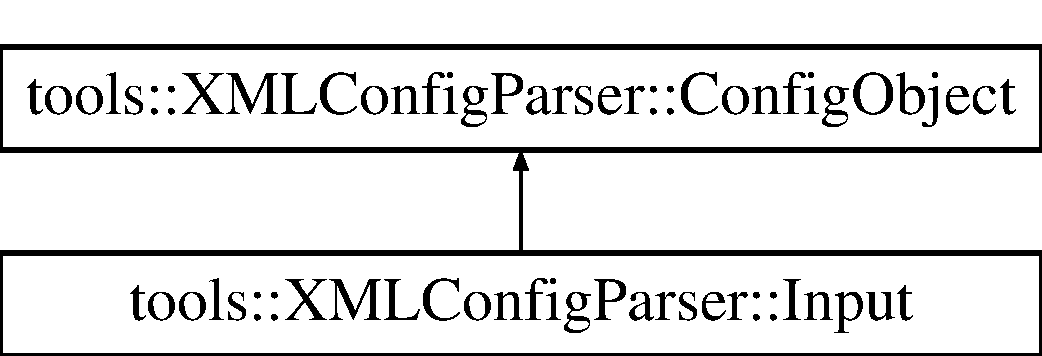
\includegraphics[height=2cm]{classtools_1_1XMLConfigParser_1_1Input}
\end{center}
\end{figure}
\subsection*{Public Member Functions}
\begin{CompactItemize}
\item 
\hypertarget{classtools_1_1XMLConfigParser_1_1Input_65cca4bf221d237f5893e547adb1a3f4}{
def \textbf{\_\-\_\-init\_\-\_\-}}
\label{classtools_1_1XMLConfigParser_1_1Input_65cca4bf221d237f5893e547adb1a3f4}

\item 
\hypertarget{classtools_1_1XMLConfigParser_1_1Input_db1d4fac10a17fadc1e2392c4181c915}{
def \textbf{setContent}}
\label{classtools_1_1XMLConfigParser_1_1Input_db1d4fac10a17fadc1e2392c4181c915}

\item 
\hypertarget{classtools_1_1XMLConfigParser_1_1Input_0bf591eb6932a4550d6c2c4bc8432a81}{
def \textbf{getFilteredContent}}
\label{classtools_1_1XMLConfigParser_1_1Input_0bf591eb6932a4550d6c2c4bc8432a81}

\end{CompactItemize}
\subsection*{Public Attributes}
\begin{CompactItemize}
\item 
\hypertarget{classtools_1_1XMLConfigParser_1_1Input_74306ef1655f005fa860125d3e809583}{
\textbf{content}}
\label{classtools_1_1XMLConfigParser_1_1Input_74306ef1655f005fa860125d3e809583}

\end{CompactItemize}
\subsection*{Static Public Attributes}
\begin{CompactItemize}
\item 
\hypertarget{classtools_1_1XMLConfigParser_1_1Input_6a1fe6d410ed958cede99812e070212f}{
string \hyperlink{classtools_1_1XMLConfigParser_1_1Input_6a1fe6d410ed958cede99812e070212f}{separator} = \char`\"{}:\char`\"{}}
\label{classtools_1_1XMLConfigParser_1_1Input_6a1fe6d410ed958cede99812e070212f}

\begin{CompactList}\small\item\em separator between shortcut and input \item\end{CompactList}\item 
\hypertarget{classtools_1_1XMLConfigParser_1_1Input_06abafad4788d8027a19cdf2f2819940}{
string \textbf{rootNodeName} = \char`\"{}input\char`\"{}}
\label{classtools_1_1XMLConfigParser_1_1Input_06abafad4788d8027a19cdf2f2819940}

\item 
list \hyperlink{classtools_1_1XMLConfigParser_1_1Input_02daa3ad92bdc203274e117a88ec8543}{doNotParse} = \mbox{[}\char`\"{}folder\char`\"{}\mbox{]}
\begin{CompactList}\small\item\em marks complex objects which have their own class. \item\end{CompactList}\item 
\hypertarget{classtools_1_1XMLConfigParser_1_1Input_d96187f7a89c6b7879473eb102622375}{
dictionary \hyperlink{classtools_1_1XMLConfigParser_1_1Input_d96187f7a89c6b7879473eb102622375}{inputTypes} = \{\char`\"{}f\char`\"{}:\char`\"{}folder\char`\"{}, \char`\"{}i\char`\"{}:\char`\"{}input\char`\"{}\}}
\label{classtools_1_1XMLConfigParser_1_1Input_d96187f7a89c6b7879473eb102622375}

\begin{CompactList}\small\item\em defines shortcuts for inputs \par
 f:foldername uses a folder as input\par
 i:inputName uses an input previously defined in the configuration file:\par
 if it is no shortcut is present the input will be interpreted as direct input (full path to histogram) \item\end{CompactList}\end{CompactItemize}


\subsection{Detailed Description}
defines an input for a histogram : does not know anything about files 

\subsection{Member Data Documentation}
\hypertarget{classtools_1_1XMLConfigParser_1_1Input_02daa3ad92bdc203274e117a88ec8543}{
\index{tools::XMLConfigParser::Input@{tools::XMLConfigParser::Input}!doNotParse@{doNotParse}}
\index{doNotParse@{doNotParse}!tools::XMLConfigParser::Input@{tools::XMLConfigParser::Input}}
\subsubsection{\setlength{\rightskip}{0pt plus 5cm}list {\bf tools::XMLConfigParser::Input::doNotParse} = \mbox{[}\char`\"{}folder\char`\"{}\mbox{]}\hspace{0.3cm}{\tt  \mbox{[}static\mbox{]}}}}
\label{classtools_1_1XMLConfigParser_1_1Input_02daa3ad92bdc203274e117a88ec8543}


marks complex objects which have their own class. 



Reimplemented from \hyperlink{classtools_1_1XMLConfigParser_1_1ConfigObject}{tools::XMLConfigParser::ConfigObject}.

The documentation for this class was generated from the following file:\begin{CompactItemize}
\item 
XMLConfigParser.py\end{CompactItemize}

\hypertarget{classtools_1_1XMLConfigParser_1_1OptionSet}{
\section{tools::XMLConfigParser::OptionSet Class Reference}
\label{classtools_1_1XMLConfigParser_1_1OptionSet}\index{tools::XMLConfigParser::OptionSet@{tools::XMLConfigParser::OptionSet}}
}
stores the options of an \hyperlink{classtools_1_1XMLConfigParser_1_1ConfigObject}{ConfigObject} and their defaults  


\subsection*{Public Member Functions}
\begin{CompactItemize}
\item 
\hypertarget{classtools_1_1XMLConfigParser_1_1OptionSet_c10781767756a542cd9c5b2beae78186}{
def \textbf{\_\-\_\-init\_\-\_\-}}
\label{classtools_1_1XMLConfigParser_1_1OptionSet_c10781767756a542cd9c5b2beae78186}

\item 
def \hyperlink{classtools_1_1XMLConfigParser_1_1OptionSet_50ceb2f5657667e4c0b3ccd71fbf0986}{getOption}
\item 
\hypertarget{classtools_1_1XMLConfigParser_1_1OptionSet_806b094a77a3f5a3d60134d23c850d26}{
def \hyperlink{classtools_1_1XMLConfigParser_1_1OptionSet_806b094a77a3f5a3d60134d23c850d26}{addOption}}
\label{classtools_1_1XMLConfigParser_1_1OptionSet_806b094a77a3f5a3d60134d23c850d26}

\begin{CompactList}\small\item\em adds an option to the \hyperlink{classtools_1_1XMLConfigParser_1_1OptionSet}{OptionSet} \item\end{CompactList}\item 
def \hyperlink{classtools_1_1XMLConfigParser_1_1OptionSet_6c3e2b6ef7030f2f9525bb52de68531d}{setDefaults}
\begin{CompactList}\small\item\em Sets the default values. \item\end{CompactList}\item 
\hypertarget{classtools_1_1XMLConfigParser_1_1OptionSet_175d8fae91a86d08e6e84c607f014128}{
def \hyperlink{classtools_1_1XMLConfigParser_1_1OptionSet_175d8fae91a86d08e6e84c607f014128}{setOptions}}
\label{classtools_1_1XMLConfigParser_1_1OptionSet_175d8fae91a86d08e6e84c607f014128}

\begin{CompactList}\small\item\em Sets the options. \item\end{CompactList}\item 
def \hyperlink{classtools_1_1XMLConfigParser_1_1OptionSet_ed3b8e8b77f780936f38389ab833f5ff}{setOption}
\begin{CompactList}\small\item\em sets an option to a value The option has to be defined in the default configuration If the option is reset a second time in one \hyperlink{classtools_1_1XMLConfigParser_1_1ConfigObject}{ConfigObject} a warning is given. \item\end{CompactList}\item 
def \hyperlink{classtools_1_1XMLConfigParser_1_1OptionSet_118681455ca2ff1e108084dd04452802}{checkOptionValue}
\begin{CompactList}\small\item\em check if the option value is allowed. \item\end{CompactList}\item 
def \hyperlink{classtools_1_1XMLConfigParser_1_1OptionSet_66effebc086caf0e5494f51502455f27}{hasOption}
\end{CompactItemize}
\subsection*{Public Attributes}
\begin{CompactItemize}
\item 
\hypertarget{classtools_1_1XMLConfigParser_1_1OptionSet_25ca2ef97315f87f05e8353ebff49537}{
\textbf{options}}
\label{classtools_1_1XMLConfigParser_1_1OptionSet_25ca2ef97315f87f05e8353ebff49537}

\item 
\hypertarget{classtools_1_1XMLConfigParser_1_1OptionSet_d17cc4d3ac989f378d3a06210775edaa}{
\textbf{defaults}}
\label{classtools_1_1XMLConfigParser_1_1OptionSet_d17cc4d3ac989f378d3a06210775edaa}

\end{CompactItemize}


\subsection{Detailed Description}
stores the options of an \hyperlink{classtools_1_1XMLConfigParser_1_1ConfigObject}{ConfigObject} and their defaults 

\subsection{Member Function Documentation}
\hypertarget{classtools_1_1XMLConfigParser_1_1OptionSet_50ceb2f5657667e4c0b3ccd71fbf0986}{
\index{tools::XMLConfigParser::OptionSet@{tools::XMLConfigParser::OptionSet}!getOption@{getOption}}
\index{getOption@{getOption}!tools::XMLConfigParser::OptionSet@{tools::XMLConfigParser::OptionSet}}
\subsubsection{\setlength{\rightskip}{0pt plus 5cm}def tools::XMLConfigParser::OptionSet::getOption ( {\em self}, \/   {\em option})}}
\label{classtools_1_1XMLConfigParser_1_1OptionSet_50ceb2f5657667e4c0b3ccd71fbf0986}


\begin{Desc}
\item[Returns:]the option with given name, if it exists. Otherwise raises \hyperlink{classtools_1_1XMLConfigParser_1_1ConfigError}{ConfigError}. \end{Desc}
\hypertarget{classtools_1_1XMLConfigParser_1_1OptionSet_6c3e2b6ef7030f2f9525bb52de68531d}{
\index{tools::XMLConfigParser::OptionSet@{tools::XMLConfigParser::OptionSet}!setDefaults@{setDefaults}}
\index{setDefaults@{setDefaults}!tools::XMLConfigParser::OptionSet@{tools::XMLConfigParser::OptionSet}}
\subsubsection{\setlength{\rightskip}{0pt plus 5cm}def tools::XMLConfigParser::OptionSet::setDefaults ( {\em self}, \/   {\em options})}}
\label{classtools_1_1XMLConfigParser_1_1OptionSet_6c3e2b6ef7030f2f9525bb52de68531d}


Sets the default values. 

\begin{Desc}
\item[\hyperlink{deprecated__deprecated000001}{Deprecated}]: will be deleted \end{Desc}
\hypertarget{classtools_1_1XMLConfigParser_1_1OptionSet_ed3b8e8b77f780936f38389ab833f5ff}{
\index{tools::XMLConfigParser::OptionSet@{tools::XMLConfigParser::OptionSet}!setOption@{setOption}}
\index{setOption@{setOption}!tools::XMLConfigParser::OptionSet@{tools::XMLConfigParser::OptionSet}}
\subsubsection{\setlength{\rightskip}{0pt plus 5cm}def tools::XMLConfigParser::OptionSet::setOption ( {\em self}, \/   {\em option}, \/   {\em value})}}
\label{classtools_1_1XMLConfigParser_1_1OptionSet_ed3b8e8b77f780936f38389ab833f5ff}


sets an option to a value The option has to be defined in the default configuration If the option is reset a second time in one \hyperlink{classtools_1_1XMLConfigParser_1_1ConfigObject}{ConfigObject} a warning is given. 

If the optionvalue is the same as the default value a warning is given \begin{Desc}
\item[Parameters:]
\begin{description}
\item[{\em option,:}]the option to change  \par
 raises \hyperlink{classtools_1_1XMLConfigParser_1_1ConfigError}{ConfigError} if option is unknown \item[{\em value,:}]the value of the option \end{description}
\end{Desc}
\hypertarget{classtools_1_1XMLConfigParser_1_1OptionSet_118681455ca2ff1e108084dd04452802}{
\index{tools::XMLConfigParser::OptionSet@{tools::XMLConfigParser::OptionSet}!checkOptionValue@{checkOptionValue}}
\index{checkOptionValue@{checkOptionValue}!tools::XMLConfigParser::OptionSet@{tools::XMLConfigParser::OptionSet}}
\subsubsection{\setlength{\rightskip}{0pt plus 5cm}def tools::XMLConfigParser::OptionSet::checkOptionValue ( {\em self}, \/   {\em option}, \/   {\em type})}}
\label{classtools_1_1XMLConfigParser_1_1OptionSet_118681455ca2ff1e108084dd04452802}


check if the option value is allowed. 

In simplest case check if string, integer or float, see typedef \hypertarget{classtools_1_1XMLConfigParser_1_1OptionSet_66effebc086caf0e5494f51502455f27}{
\index{tools::XMLConfigParser::OptionSet@{tools::XMLConfigParser::OptionSet}!hasOption@{hasOption}}
\index{hasOption@{hasOption}!tools::XMLConfigParser::OptionSet@{tools::XMLConfigParser::OptionSet}}
\subsubsection{\setlength{\rightskip}{0pt plus 5cm}def tools::XMLConfigParser::OptionSet::hasOption ( {\em self}, \/   {\em option})}}
\label{classtools_1_1XMLConfigParser_1_1OptionSet_66effebc086caf0e5494f51502455f27}


\begin{Desc}
\item[Returns:]: if option is in the set \end{Desc}


The documentation for this class was generated from the following file:\begin{CompactItemize}
\item 
XMLConfigParser.py\end{CompactItemize}

\hypertarget{classtools_1_1PadService_1_1PadService}{
\section{tools::PadService::PadService Class Reference}
\label{classtools_1_1PadService_1_1PadService}\index{tools::PadService::PadService@{tools::PadService::PadService}}
}
builds canvas up to 6 hists  


\subsection*{Public Member Functions}
\begin{CompactItemize}
\item 
\hypertarget{classtools_1_1PadService_1_1PadService_1a9f48ad85e894de996666ca2c6e1f9d}{
def \textbf{\_\-\_\-init\_\-\_\-}}
\label{classtools_1_1PadService_1_1PadService_1a9f48ad85e894de996666ca2c6e1f9d}

\item 
\hypertarget{classtools_1_1PadService_1_1PadService_273e402a3566dc6818fe681e1c3b4a0c}{
def \textbf{Next}}
\label{classtools_1_1PadService_1_1PadService_273e402a3566dc6818fe681e1c3b4a0c}

\end{CompactItemize}
\subsection*{Public Attributes}
\begin{CompactItemize}
\item 
\hypertarget{classtools_1_1PadService_1_1PadService_166437daa5e84fa12b931260cdadd5aa}{
\textbf{nPadsX}}
\label{classtools_1_1PadService_1_1PadService_166437daa5e84fa12b931260cdadd5aa}

\item 
\hypertarget{classtools_1_1PadService_1_1PadService_699b146575aa9184cdc43d4770461597}{
\textbf{nPadsY}}
\label{classtools_1_1PadService_1_1PadService_699b146575aa9184cdc43d4770461597}

\item 
\hypertarget{classtools_1_1PadService_1_1PadService_0c356b6b9df540ca9b4ef4892429b138}{
\textbf{width}}
\label{classtools_1_1PadService_1_1PadService_0c356b6b9df540ca9b4ef4892429b138}

\item 
\hypertarget{classtools_1_1PadService_1_1PadService_ae38b59241fa933587eda646096cbf84}{
\textbf{height}}
\label{classtools_1_1PadService_1_1PadService_ae38b59241fa933587eda646096cbf84}

\item 
\hypertarget{classtools_1_1PadService_1_1PadService_6afe4249db1b2c3a4ca4ec847b3cf15d}{
\textbf{last}}
\label{classtools_1_1PadService_1_1PadService_6afe4249db1b2c3a4ca4ec847b3cf15d}

\item 
\hypertarget{classtools_1_1PadService_1_1PadService_6d4eb6e42e6ce64cfcdc06b0ca813786}{
\textbf{index}}
\label{classtools_1_1PadService_1_1PadService_6d4eb6e42e6ce64cfcdc06b0ca813786}

\item 
\hypertarget{classtools_1_1PadService_1_1PadService_e804fe4aa16cd6234a2e85a85cd290ad}{
\textbf{count}}
\label{classtools_1_1PadService_1_1PadService_e804fe4aa16cd6234a2e85a85cd290ad}

\item 
\hypertarget{classtools_1_1PadService_1_1PadService_c0584edaec9da3268746adf851a7f6c3}{
\textbf{name}}
\label{classtools_1_1PadService_1_1PadService_c0584edaec9da3268746adf851a7f6c3}

\item 
\hypertarget{classtools_1_1PadService_1_1PadService_d68d6735dbba044c6406d99325adc839}{
\textbf{title}}
\label{classtools_1_1PadService_1_1PadService_d68d6735dbba044c6406d99325adc839}

\end{CompactItemize}


\subsection{Detailed Description}
builds canvas up to 6 hists 

The documentation for this class was generated from the following file:\begin{CompactItemize}
\item 
PadService.py\end{CompactItemize}

\hypertarget{classtools_1_1testConfigParser_1_1testConfigParser}{
\section{tools::testConfigParser::testConfigParser Class Reference}
\label{classtools_1_1testConfigParser_1_1testConfigParser}\index{tools::testConfigParser::testConfigParser@{tools::testConfigParser::testConfigParser}}
}
A test class for the ConfigParser module.  


\subsection*{Public Member Functions}
\begin{CompactItemize}
\item 
\hypertarget{classtools_1_1testConfigParser_1_1testConfigParser_c26e240cf3a5b3224ba506e1358c2cb9}{
def \textbf{setUp}}
\label{classtools_1_1testConfigParser_1_1testConfigParser_c26e240cf3a5b3224ba506e1358c2cb9}

\item 
\hypertarget{classtools_1_1testConfigParser_1_1testConfigParser_c9719900350ddc7bf1905387746952fa}{
def \textbf{testInit}}
\label{classtools_1_1testConfigParser_1_1testConfigParser_c9719900350ddc7bf1905387746952fa}

\item 
\hypertarget{classtools_1_1testConfigParser_1_1testConfigParser_4eaa44ca2d5be3ba1c2812bdcccb7521}{
def \textbf{testGetRoot}}
\label{classtools_1_1testConfigParser_1_1testConfigParser_4eaa44ca2d5be3ba1c2812bdcccb7521}

\item 
\hypertarget{classtools_1_1testConfigParser_1_1testConfigParser_92abba78db68f7e6f7cf994c6833dff1}{
def \textbf{testGetNodeList}}
\label{classtools_1_1testConfigParser_1_1testConfigParser_92abba78db68f7e6f7cf994c6833dff1}

\item 
\hypertarget{classtools_1_1testConfigParser_1_1testConfigParser_b49d7cff8744c74f75034419ccb212f5}{
def \textbf{testGetAttributeValue}}
\label{classtools_1_1testConfigParser_1_1testConfigParser_b49d7cff8744c74f75034419ccb212f5}

\item 
\hypertarget{classtools_1_1testConfigParser_1_1testConfigParser_d12ec88da937a6aff7329b88e4bd5c7d}{
def \textbf{testReadIncludes}}
\label{classtools_1_1testConfigParser_1_1testConfigParser_d12ec88da937a6aff7329b88e4bd5c7d}

\item 
\hypertarget{classtools_1_1testConfigParser_1_1testConfigParser_f0bea5527c82fbf480aec857d6f61ffb}{
def \textbf{testGetInputFiles}}
\label{classtools_1_1testConfigParser_1_1testConfigParser_f0bea5527c82fbf480aec857d6f61ffb}

\item 
\hypertarget{classtools_1_1testConfigParser_1_1testConfigParser_00275c52d0b09941b65333731ebc2a0a}{
def \textbf{testGetInputs}}
\label{classtools_1_1testConfigParser_1_1testConfigParser_00275c52d0b09941b65333731ebc2a0a}

\item 
\hypertarget{classtools_1_1testConfigParser_1_1testConfigParser_6bd781de57ff3093664b65301839068d}{
def \textbf{testGetChildNodes}}
\label{classtools_1_1testConfigParser_1_1testConfigParser_6bd781de57ff3093664b65301839068d}

\item 
\hypertarget{classtools_1_1testConfigParser_1_1testConfigParser_192206b692e12b004c0119fa0428f8b3}{
def \textbf{testGetPlots}}
\label{classtools_1_1testConfigParser_1_1testConfigParser_192206b692e12b004c0119fa0428f8b3}

\item 
\hypertarget{classtools_1_1testConfigParser_1_1testConfigParser_9d20d3c076b5dd3f5f6d13afb98e7380}{
def \textbf{testGetFilenameByID}}
\label{classtools_1_1testConfigParser_1_1testConfigParser_9d20d3c076b5dd3f5f6d13afb98e7380}

\item 
\hypertarget{classtools_1_1testConfigParser_1_1testConfigParser_99e009490067d0fe5f74fc9a109e1e93}{
def \textbf{testFileContainsHist}}
\label{classtools_1_1testConfigParser_1_1testConfigParser_99e009490067d0fe5f74fc9a109e1e93}

\end{CompactItemize}
\subsection*{Public Attributes}
\begin{CompactItemize}
\item 
\hypertarget{classtools_1_1testConfigParser_1_1testConfigParser_2c801c8beb4faf426081fc54a31a1c20}{
\textbf{testxml}}
\label{classtools_1_1testConfigParser_1_1testConfigParser_2c801c8beb4faf426081fc54a31a1c20}

\item 
\hypertarget{classtools_1_1testConfigParser_1_1testConfigParser_568a2ad22e901ef1a5cfd6d7df642df2}{
\textbf{falsexml}}
\label{classtools_1_1testConfigParser_1_1testConfigParser_568a2ad22e901ef1a5cfd6d7df642df2}

\item 
\hypertarget{classtools_1_1testConfigParser_1_1testConfigParser_ceed80dc45bd57e8304c9c20716c8fa3}{
\textbf{parser}}
\label{classtools_1_1testConfigParser_1_1testConfigParser_ceed80dc45bd57e8304c9c20716c8fa3}

\item 
\hypertarget{classtools_1_1testConfigParser_1_1testConfigParser_ee33eeddbb65528094b4328b3298e963}{
\textbf{falseParser}}
\label{classtools_1_1testConfigParser_1_1testConfigParser_ee33eeddbb65528094b4328b3298e963}

\end{CompactItemize}


\subsection{Detailed Description}
A test class for the ConfigParser module. 

called after constructor, sets the variables 

The documentation for this class was generated from the following file:\begin{CompactItemize}
\item 
testConfigParser.py\end{CompactItemize}

\hypertarget{classtools_1_1testXMLParser_1_1TestParser}{
\section{tools::testXMLParser::TestParser Class Reference}
\label{classtools_1_1testXMLParser_1_1TestParser}\index{tools::testXMLParser::TestParser@{tools::testXMLParser::TestParser}}
}
TestCase for the XMLConfigParser.  




\subsection{Detailed Description}
TestCase for the XMLConfigParser. 

The documentation for this class was generated from the following file:\begin{CompactItemize}
\item 
testXMLParser.py\end{CompactItemize}

\printindex
\end{document}
